\documentclass[11pt]{article}
\usepackage[margin=1in]{geometry}
\usepackage{amsmath,amsthm,amssymb}
\usepackage{float}
\usepackage{hyperref}
\usepackage{booktabs}
\usepackage{placeins}
\usepackage{graphicx}
\usepackage[
backend=biber,
style=bwl-FU,
sorting=ynt
]{biblatex}
\addbibresource{main.bib}

\DeclareMathOperator*{\argmax}{arg\,max}
\DeclareMathOperator*{\argmin}{arg\,min}

\title{Single Zone Evaluation}
\author{José I. Velarde Morales}

\begin{document}
\maketitle

\section{Setup}
    \subsection*{Data Generating Process}
    We use the following data generating processes for the toy examples. In order to make the comparison with the status quo more straightforward, we model losses instead of overall wealth. 
    \begin{align*}
        l&=\beta \theta + \epsilon\\
        \theta &\sim \mathcal{N}(5,2)\\
        \epsilon &\sim \mathcal{N}(0,1)\\
        \beta &= 3
    \end{align*}
    I draw 100 training samples from the above model to train the prediction model and to use as input for the optimization programs. I then evaluate both methods using 1000 samples drawn from the same model. 

\section{Status Quo}
We will be comparing our proposed approach to the method developed by \cite{chantarat2013designing}, which, to the extent of our knowledge is what is currently being used for Kenya's Index Based Livestock Insurance (IBLI) program. The method is as follows: 
\begin{itemize}
    \item First, they use a clustering algorithm to group locations into clusters
    \item They then use historical data to fit a linear regression model to predict herd mortality rates in each cluster. They fit a different model for each cluster. 
    \item Contracts are of the form: $I(\theta) = \max(\hat{M}(\theta)-M^*,0)\times TLU \times P_{TLU}$ where $\hat{M}(\theta)$ is the predicted herd mortality rate, $M^*$ is the strike value, $TLU$ is the number of insured livestock units, and $P_{TLU}$ is the price per insured livestock unit.  In other words, their contract pays farmers for the full predicted loss beyond a threshold, $M^*$. This threshold, $M^*$ is the contract's strike value. 
    \item They choose the strike value that would explain the highest share of insurable losses in the historical data. Specifically, they run the following regression: $y_s = \beta_s \hat{y_s}+\epsilon$ where $y_s$ is the actual insured losses at strike value $s$ and $\hat{y_s}$ is the predicted insured losses at strike value $s$. For example, suppose that $TLU=100$ (ie there are 100 insured units), and that $P_{TLU}=25$ (ie each unit is worth 25), and that $M^* = 0.25$ (ie contract starts paying out once the predicted mortality rate exceeds $25\%$). If the actual mortality rate is $0.5$, then actual insured losses would be $y_{25} = \max(M-M^*,0)\times TLU \times P_{TLU} = (0.5-0.25)\times(100) \times (25)$. If the predicted mortality rate in that scenario was $0.4$, the predicted insured losses, $\hat{y_{25}} = \max(\hat{M}(\theta)-M^*,0)\times TLU \times P_{TLU} = (0.4-0.25)\times(100) \times (25)$. They use historical data to calculate $y_s, \hat{y_s}$, and then run the following regression: $y_s = \beta_s \hat{y_s}+\epsilon$. They choose the strike value $s= \argmax_s \beta_s$. This takes into account the fact that the prediction model, $\hat{M}(\theta)$ might be better at predicting some losses better than others. 
\end{itemize}

To mimick this in our toy example, we set the status quo contracts to be $I(\theta) = \max(\hat{l}(\theta)-l^*,0)$, since we are already assuming that $l$ is the total loss suffered. For the toy example, we fit a (correctly specified) linear regression model to predict losses: $l = \beta \theta + \epsilon \implies \hat{l}(\theta) = \hat{\beta}\theta$. 

\section{Optimization Approach}
In order to separate the effect of contract design from the effect of prediction quality, we will be basing our contracts on the same predictions used by the status quo method. In other words, we will use the status quo method to estimate a model that predicts loss based on theta, $\hat{l}(\theta)$, and our payout function will use that as input instead of $\theta$. In other words, our model will define payout functions $I(\hat{l}(\theta))$, where $\hat{l}(\theta)$ is the same prediction function used by the status quo method. 

\subsection*{Minimum CVaR Model}
    This model minimizes the $CVaR$ of the farmer's net loss subject to a constraint on the premium. The premium constraints are expressed as a fraction of the full insured amount. 
    \paragraph*{Model Parameters}
    \begin{itemize}
        \item $\epsilon$: This defines the CVaR objective. $\epsilon = 0.1$ means that our objective is on the expected value of the loss given that it is above the $90^{th}$ percentile. 
        \item $\bar{\pi}$: This is the maximum value of the premium. 
        \item $y$: maximum insured amount
    \end{itemize}

    \subsubsection*{Single Zone Model}

    \begin{align}
        \min_{a,b\geq 0} &\ CV@R_{1-\epsilon}\left(\ell  - \min\left\{(a\theta + b), K\right\} \right)\\
        \text{s.t.   } &\   a \mathbb{E} \left[\theta \right] + b\label{eq-02} \leq \bar{\pi}\\
        & a\theta + b \geq 0 
    \end{align}

    We reformulated the problem in the following way. In the model below, $p_k$ is the probability of event $k$, and $k$ indexes the possible realizations of $\theta, l$.

    \begin{align}
        \min_{a,b,\pi,\gamma,t} &\quad t + \frac{1}{\epsilon}\sum_k p_k \gamma_k\\
        \text{s.t.   } \gamma_k &\geq l^k - \min\left\{(a\hat{l}(\theta^k) + b), K\right\} - t, \forall k\\
        \gamma_k &\geq 0, \forall k \\
        0 &\leq a\hat{l}(\theta^k) + b, \forall k\\
        K\bar{\pi} &\geq a\mathbb{E}[\hat{l}(\theta)] + b
    \end{align}

\section{Results}
The model mostly behaves as expected. Increasing the payment cap, $K$ increases $a$ and decreases $b$, in other words, it increases the slope of the payout function and shifts it right. Similarly, increasing the maximum premium, $\bar{\pi}$ increases the payout rate and shifts it right as well. However, $a$ and $b$ didn't seem sensitive to $\epsilon$ at all. I think this is because the data generating process is linear, $\ell = \beta \theta + \epsilon$. When I replace that data generating process with a cubic one, $\ell = \beta \theta^3 + \epsilon$, $a,b$ become sensitive to $\epsilon$. In general, as $\epsilon$ decreases, $a$ increases and $b$ decreases, which I think is the behavior we would expect, because it would be more targeted towards losses at the right tail of the distribution. 
    \subsection*{CVaR Model}
        \subsubsection*{Max Premium Exploration}
        \begin{figure}[H]
            \centering
            \caption{Max Premium Exploration}
            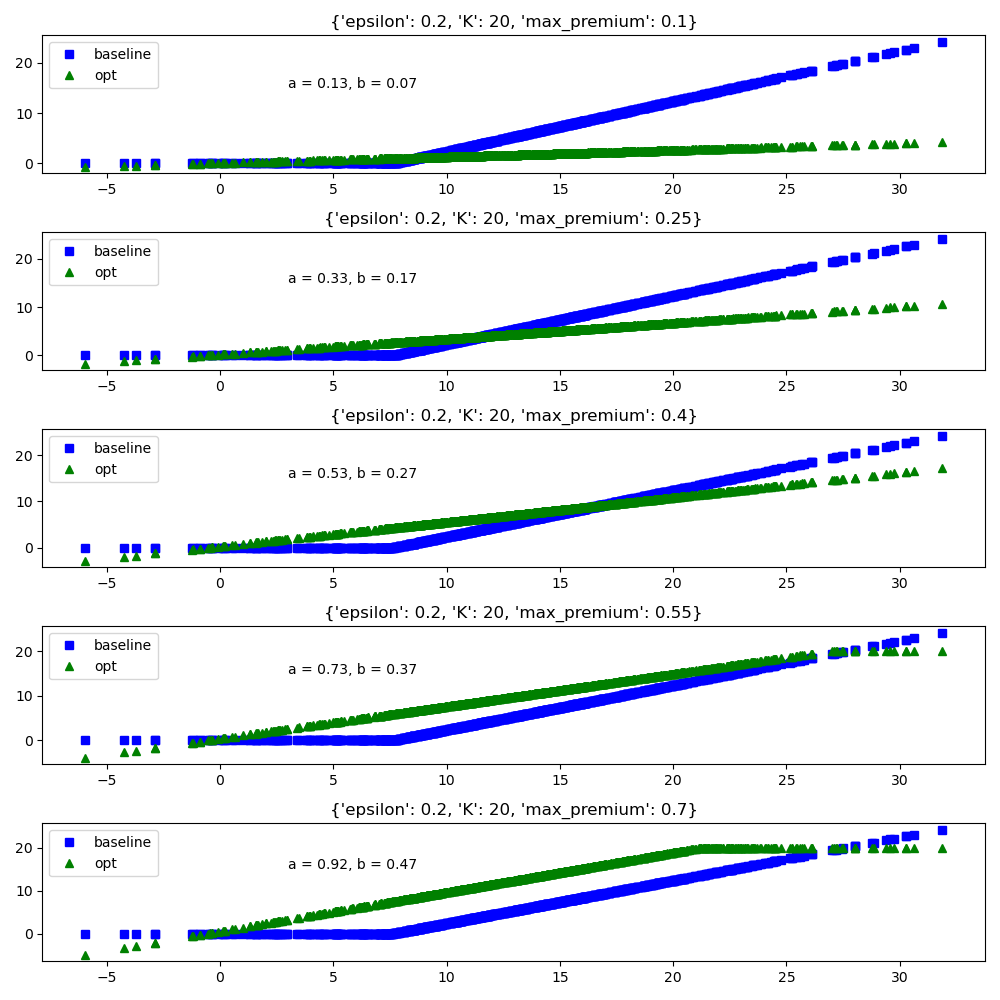
\includegraphics[width=0.75\textwidth]{../../output/figures/CVaR3/max_premium_exploration.png}
        \end{figure}

        % \begin{table}[H]
        %     \centering
        %     \caption{Performance Metrics}
        %     \begin{tabular}{lrrrrrl}
\toprule
{} &  \$P(L > 70)\$ &  \$P(L > 80)\$ &  \$P(L > 90)\$ &  \$P(L > 95)\$ &  Premium & max\_premium \\
\midrule
0 &         0.16 &         0.08 &         0.03 &         0.01 &     2.01 &         0.1 \\
2 &         0.02 &         0.00 &         0.00 &         0.00 &     4.78 &        0.25 \\
4 &         0.00 &         0.00 &         0.00 &         0.00 &     7.72 &         0.4 \\
6 &         0.00 &         0.00 &         0.00 &         0.00 &    10.61 &        0.55 \\
8 &         0.00 &         0.00 &         0.00 &         0.00 &    13.11 &         0.7 \\
1 &         0.00 &         0.00 &         0.00 &         0.00 &     6.68 &    Baseline \\
\bottomrule
\end{tabular}

        % \end{table}

        \FloatBarrier

        \subsubsection*{K Exploration}
        \begin{figure}[H]
            \centering
            \caption{K Exploration}
            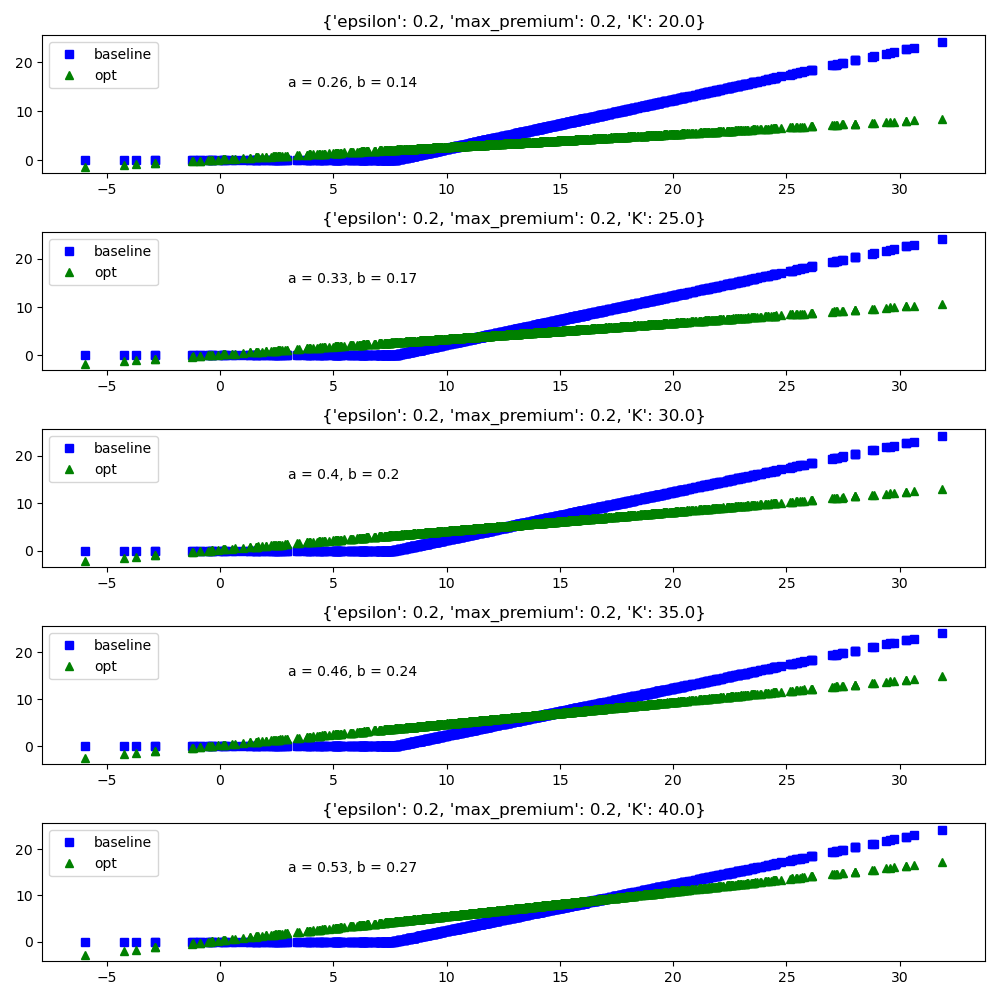
\includegraphics[width=0.75\textwidth]{../../output/figures/CVaR3/K_exploration.png}
        \end{figure}

        % \begin{table}[H]
        %     \centering
        %     \caption{Performance Metrics}
        %     \begin{tabular}{lrrrrlr}
\toprule
{} &  \$P(L > 70)\$ &  \$P(L > 80)\$ &  \$P(L > 90)\$ &  \$P(L > 95)\$ &         K &  Premium \\
\midrule
0 &         0.07 &         0.03 &         0.01 &         0.00 &      20.0 &     3.71 \\
2 &         0.03 &         0.01 &         0.00 &         0.00 &      25.0 &     4.70 \\
4 &         0.01 &         0.00 &         0.00 &         0.00 &      30.0 &     5.69 \\
6 &         0.00 &         0.00 &         0.00 &         0.00 &      35.0 &     6.56 \\
8 &         0.00 &         0.00 &         0.00 &         0.00 &      40.0 &     7.55 \\
1 &         0.00 &         0.00 &         0.00 &         0.00 &  Baseline &     6.50 \\
\bottomrule
\end{tabular}

        % \end{table}

        \FloatBarrier

        \subsubsection*{Epsilon Exploration}
            \begin{figure}[H]
                \centering
                \caption{Epsilon Exploration}
                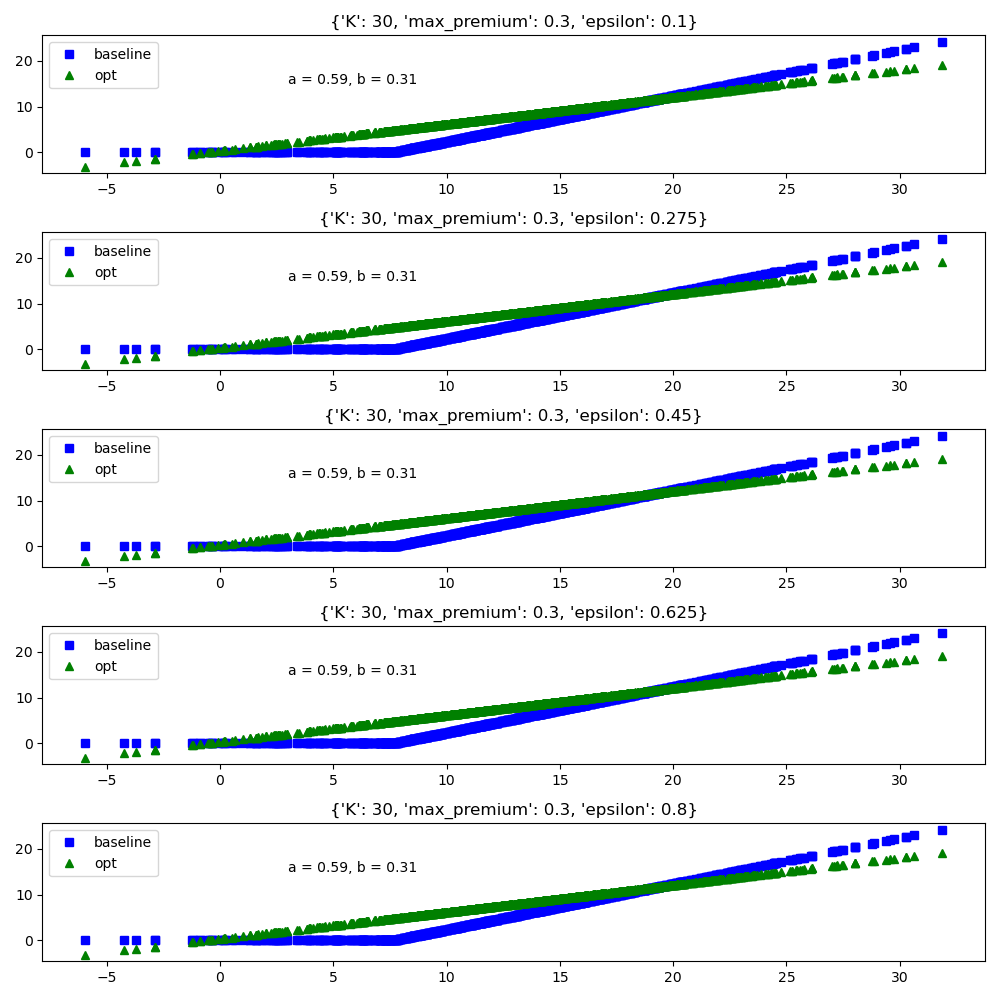
\includegraphics[width=0.75\textwidth]{../../output/figures/CVaR3/epsilon_exploration.png}
            \end{figure}

            % \begin{table}[H]
            %     \centering
            %     \caption{Performance Metrics}
            %     \begin{tabular}{lrrrrrl}
\toprule
{} &  \$P(L > 70)\$ &  \$P(L > 80)\$ &  \$P(L > 90)\$ &  \$P(L > 95)\$ &  Premium &   epsilon \\
\midrule
0 &         0.00 &         0.00 &         0.00 &         0.00 &     8.64 &       0.1 \\
2 &         0.00 &         0.00 &         0.00 &         0.00 &     8.64 &     0.275 \\
4 &         0.00 &         0.00 &         0.00 &         0.00 &     8.64 &      0.45 \\
6 &         0.00 &         0.00 &         0.00 &         0.00 &     8.64 &     0.625 \\
8 &         0.00 &         0.00 &         0.00 &         0.00 &     8.64 &       0.8 \\
1 &         0.00 &         0.00 &         0.00 &         0.00 &     6.68 &  Baseline \\
\bottomrule
\end{tabular}

            % \end{table}

            \FloatBarrier









% \section*{Baseline Approach}
% We will be comparing our proposed approach to the method developed by \cite{chantarat2013designing}, which, to the extent of our knowledge is what is currently being used for Kenya's Index Based Livestock Insurance (IBLI) program. The method is as follows: 
% \begin{itemize}
%     \item Cluster locations into two clusters
%     \item Fit a separate herd mortality function for each cluster. They use a linear regression model to predict herd mortality. 
%     \item Contracts are offered at the cluster level, but payouts are at the location level. 
%     \item They choose the strike level that would explain the highest share of insurable losses in the historical data. 
% \end{itemize}

% \section*{Toy Examples}
% \subsection*{Data Generating Process}
% We use the following data generating processes for the toy examples. In order to make the comparison with the status quo more straightforward, we model losses instead of overall wealth. 
% \begin{itemize}
%     \item $l=\beta \theta + \epsilon$ where $w,\theta \in \mathbb{R}^z$ where $z$ is the number of zones, and $\theta \sim \mathcal{N}(\mu,\Sigma), \epsilon \sim \mathcal{N}(0,\sigma I)$.
%     \item $l= f(\theta) + \epsilon$ where $\theta \sim \mathcal{N}(\mu,\Sigma)$, $f$ is nonlinear, and $\epsilon \sim \mathcal{N}(0,\sigma I)$.
% \end{itemize}

% \subsection*{Performance Metrics}
% We will be using the following performance metrics to compare the two approaches. 
% \begin{itemize}
%     \item Accuracy: percentage of correct decisions (i.e. giving a payout when a covered loss occured, and not giving a payout when a covered loss does not occur.)
%     \item Insurer Basis Risk: probability that the contract will pay out when a covered loss did not occur.
%     \item Insured Party Basis Risk: probability that the contract will not pay out when a covered loss occurs. 
%     \item Probability of farmer ruin: probability that loss net of insurance exceeds a pre-specified threhsold.
%     \item Cost to insurer: average cost to insurer, should also include extreme cases. 
%     \item Share of losses covered
% \end{itemize}

%   \subsection*{Parameter Values}
%     Since we will be using a simplified model in the toy examples, we will only need to set three parameters. We describe how we set each one below. 
%     \begin{itemize}
%         \item $\bar{w}$: This is the wealth threshold we want farmers to be above. We will set this to be the $10^{th}$ percentile of the distribution of $w$ for now. In the future, this should probably be determined by the setting, and what would be considered catastrophic in each setting. 
%         \item $c_K$: This is the cost of capital, and there are estimates available (e.g. \href{https://pages.stern.nyu.edu/~adamodar/New_Home_Page/datafile/wacc.html}{here}). According to this source, the average cost of capital for general insurance companies was $4.66\%$. 
%         \item $\beta_z$: This is the relative riskiness of each zone. For now, we will set $\beta_z = \frac{1-R^2_z}{\sum_z 1-R^2_z}$. 
%     \end{itemize}

%   \subsection*{1 Zone Case}
%     \subsubsection*{Data Generating Process}
%       In the one zone case, we will generate 1,100 samples from the model: $w = \beta \theta + \epsilon$, with $\theta \sim \mathcal{N}(5,10), \beta = 2, \epsilon \sim \mathcal{N}(0,1)$. 80 samples will be used for training, 20 for model selection, and 1000 for evaluation.

%     \subsubsection*{Baseline Approach for 1 zone case}
%         In the one zone case, we will replicate the baseline approach as follows: 
%         \begin{enumerate}
%             \item We will fit a linear model to the simulated data of $w, \theta$. This model will generate predictions, $\hat{w}(\theta)$
%             \item The insurance contract will be of the form $(\hat{w}(\theta) - w^*)^+$, where $w^*$ will be decided according to the share of losses covered in the hold out set. 
%         \end{enumerate}

%     \subsubsection*{Optimization Approach for 1 zone case}
%         For the single zone case, we will be solving the following model, with $\bar{w}$ set to the $20^{th}$ percentile of the empirical distribution of $w$. In order to separate the effect from the design of the contract from the design of the index, we will use the same index, $\hat{w}(\theta)$ as in the baseline approach.
%         \begin{align}
%             \min_{a,d,\pi} & E[I^k]\\
%             \text{s.t.   } I^k &= a\hat{w}(\theta^k) + d, \forall k\\
%             0 &\leq I^k, \forall k\\
%             t + \frac{1}{\epsilon}&\sum_k p_k \gamma_k \leq 0\\
%             \gamma_k &\geq \bar{w}-w^k + E[I] -I^k -t, \forall k\\
%             \gamma_k &\geq 0, \forall k
%         \end{align}

%   \subsection*{2 Zone Case}
%     \subsubsection*{Data Generating Process}
%     In the two zone case, we will generate 1,100 samples from the model: $w = \beta \theta + \epsilon$, with $\theta \sim \mathcal{N}((3,5),\Sigma), \beta = (1.5,2), \epsilon \sim \mathcal{N}(0,I)$. 80 samples will be used for training, 20 for model selection, and 1000 for evaluation. We will use the two following options:
%     \begin{itemize}
%         \item $\Sigma$ s.t. $Corr(\theta_1,\theta_2)=0.6$
%         \item $\Sigma$ s.t. $Corr(\theta_1,\theta_2)=-0.6$
%     \end{itemize}

%     \subsubsection*{Baseline Approach for 2 zone case}
%         In the one zone case, we will replicate the baseline approach as follows: 
%         \begin{enumerate}
%             \item We will fit a linear model to the simulated data of $w, \theta$. This model will generate predictions, $\hat{w}(\theta)$
%             \item The insurance contract will be of the form $(\hat{w}(\theta) - w^*)^+$, where $w^*$ will be decided according to the share of losses covered in the hold out set. 
%         \end{enumerate}

%     \subsubsection*{Optimization Approach for 2 zone case}
%         For the single zone case, we will be solving the following model, with $\bar{w}$ set to the $20^{th}$ percentile of the empirical distribution of $w$. In order to separate the effect from the design of the contract from the design of the index, we will use the same index, $\hat{w}(\theta)$ as in the baseline approach.
%         \begin{align}
%             \min_{a,b,\pi} \max_z \pi_z\\
%             \text{s.t.   } I_z^k &= a_z\hat{w}(\theta^k_z) +b_z, \forall k, \forall z\\
%             0 &\leq I_z^k \leq y_z, \forall k, \forall z \\
%             t_z &+ \frac{1}{\epsilon} \sum_{k=1}^K p_k \gamma_z^k \leq 0, \forall z \\
%             \gamma_z^k &\geq \bar{w} -w_z^k + \pi_z -I_z^k -t_z, \forall k, \forall z\\
%             \gamma_z^k &\geq 0, \forall k, \forall z\\
%             t_P &+ \frac{1}{\epsilon_P} \sum_{k=1}^K p_k \gamma_P^k \leq K^P + Z \bar{\pi}\\
%             \gamma_P^k &\geq \sum_z I_z^k -t_P\\
%             \gamma_P^k &\geq 0, \forall k\\
%             \pi_z &= E[I_z]+c_K K^P\beta_z
%         \end{align}
    
% \section*{Data-Based Evaluation}
%   \subsection*{Data Sources}
%     We will be using three main data sources for the empirical evaluation of our method. These sources are: 
%     \begin{itemize}
%         \item NDVI Data: Normalized Difference Vegetation Index data. These are satellite images of the vegetation in the insured area. 
%     \end{itemize}

%   \subsection*{Simulation Procedure}

%   \subsection*{Performance Metrics}

\end{document}